\documentclass{article}
\usepackage{iclr2026_conference,times}
\input{math_commands.tex}

\usepackage{amsmath,amssymb}
\usepackage{booktabs}
\usepackage{graphicx}
\usepackage{hyperref}
\usepackage{microtype}
\usepackage{tikz}
\usepackage{url}

\hypersetup{colorlinks=true,linkcolor=blue,citecolor=blue,urlcolor=blue}

\title{Local Personal Cards for Cross-Session Preference Transfer to Frozen Language Models}
\author{Anonymous Authors}

\begin{document}
\maketitle

\begin{abstract}
A user's chat history contains useful preference signals, but sending that history
to a remote language model exposes more personal data than the model needs.
We study a local alternative. A Qwen3-0.6B model with a LoRA adapter reads past
tasks, assistant answers, and explicit user corrections on the user's machine.
It emits schema-validated \emph{Personal Cards} that record task type, feedback
facets, preference direction, confidence, scope, and a short instruction. A
deterministic profile builder transfers a rule only when the same instruction is
supported by at least two distinct records. A frozen Sonnet 4.5 model then
receives the current task and this compact profile, but not the earlier
conversations or card evidence text.

We train the local extractor on 914 examples from one user's archive. On 183
conversation-disjoint test examples, the adapter produces valid card JSON for
every input, with 0.705 task-type accuracy and 0.732 feedback micro F1. The
untouched base model produces no valid card under the same prompt and decoding
protocol; this is a structural control rather than a strong baseline. A
single-card transfer diagnostic shows no advantage. With repeated support,
the profile wins 5 of 7 position-consistent comparisons on eight new tasks.
Mean task quality is unchanged at 4.25, while mean preference fit rises from
3.375 to 4.0. However, paired bootstrap intervals for both deltas include
zero. These results show that the full local-extraction and remote-transfer
loop is feasible, not that it yields a reliable personalization gain. The
study covers one user, uses the same model family as executor and judge, and
offers data minimization rather than a formal privacy guarantee.
\end{abstract}

\section{Introduction}
\label{sec:introduction}

A correction such as ``give me a table, not another long explanation'' can be
useful beyond the conversation in which it appeared. The obvious solution is
to retrieve the earlier exchange and place it in the next model prompt. That
also sends the old task, answer, and feedback to the remote provider.

We ask a narrower question: can a small local model turn past corrections into
a compact profile that helps a frozen remote model on later tasks? The local
model may read the sensitive history. The remote model may receive the current
task and a short derived profile, but not the old conversations.

Our system has three steps. First, deterministic rules build supervised
examples from one user's archive. Second, a locally trained Qwen3-0.6B
extractor maps each observation to a structured Personal Card. Third, a local
SQLite store groups cards by exact instruction and transfers only repeatedly
supported rules. The remote Sonnet 4.5 executor is never fine-tuned. It is
guided through its normal system-prompt interface.

This split is useful for closed models. Personalized fine-tuning changes the
model that produces the answer \citep{li2024personalizedrlhf}; soft-prompt and
decoding-time methods need embedding or logit access
\citep{hebert2024persoma,lv2025costeer}. Our executor exposes neither. A
readable text profile works with the same interface used by a command-line
agent or hosted assistant.

The evidence is deliberately small. The archive represents one user, and the
online comparison has eight tasks. We therefore report the negative
single-card run, the positive point estimate from repeated support, both
zero-crossing bootstrap intervals, and concrete failures. Our contributions
are:
\begin{itemize}
    \item a fixed Personal Card schema and three-way evidence contract for
    explicit corrections, verified revisions, and category-only abstentions;
    \item a local 0.6B extractor trained on 914 archive examples, with
    conversation-disjoint evaluation and a complete H100 training record;
    \item a repeated-support profile builder that blocks one-off rules and
    exposes its ranking and transfer metadata;
    \item an order-reversed cross-session evaluation with task quality,
    preference fit, uncertainty, latency, cost, and failure analysis.
\end{itemize}

\section{Related Work}
\label{sec:related}

\paragraph{Preferences from feedback and edits.}
P-RLHF learns personalized language or reward models from user-specific
feedback \citep{li2024personalizedrlhf}. CIPHER is closer to our data source:
it infers preferences from user edits and reuses them for later contexts
\citep{gao2024cipher}. Our remote executor remains frozen, while a separate
small model extracts a discrete local record. The repeated-support rule also
blocks a correction that appears only once.

\paragraph{Personalization at the model interface.}
PERSOMA compresses history into learned soft prompts
\citep{hebert2024persoma}. CoSteer changes a cloud model's token distribution
during decoding with a local delta model \citep{lv2025costeer}. Both are more
expressive than plain text, but they need access that a prompt-only API does
not expose. Personal Cards use ordinary text and can be inspected or deleted
before use. LaMP studies retrieval-based personalization across users and
tasks \citep{salemi2023lampwl}. General memory systems such as MemGPT and Mem0
also carry information across sessions \citep{packer2023memgpttl,chhikara2025mem0bp}.
Our focus is narrower: reduce the old conversation to a short preference
artifact before the remote call.

\paragraph{Evaluation.}
LLM judges show position bias, so we judge each answer pair in both orders
\citep{zheng2023judginglw}. They can also favor generations from their own
model family \citep{panickssery2024llmer}. We cannot remove that risk because
Sonnet 4.5 is both executor and judge, but we state it and report every
order-inconsistent pair. We use paired bootstrap intervals to show the large
uncertainty from eight tasks \citep{efron1979bootstrapma}.

\section{Method}
\label{sec:method}

\subsection{Local and Remote Roles}

Let an historical observation be
\[
o=(x,a,f,r),
\]
where $x$ is the earlier task, $a$ is the assistant answer, $f$ is the
user's feedback, and $r$ records whether a revised answer passed a local
deterministic check. The local extractor $E_\theta$ returns a Personal Card
$c=E_\theta(o)$. The remote executor $R$ receives a new task $x'$ and,
in the guided condition, a rendered profile $P_\tau$ for task type $\tau$:
\[
y_{\mathrm{base}}=R(x'), \qquad
y_{\mathrm{profile}}=R(P_\tau,x').
\]
The remote executor never receives $o$ or the card's evidence sentence.

\begin{figure}[t]
\centering
\resizebox{\linewidth}{!}{%
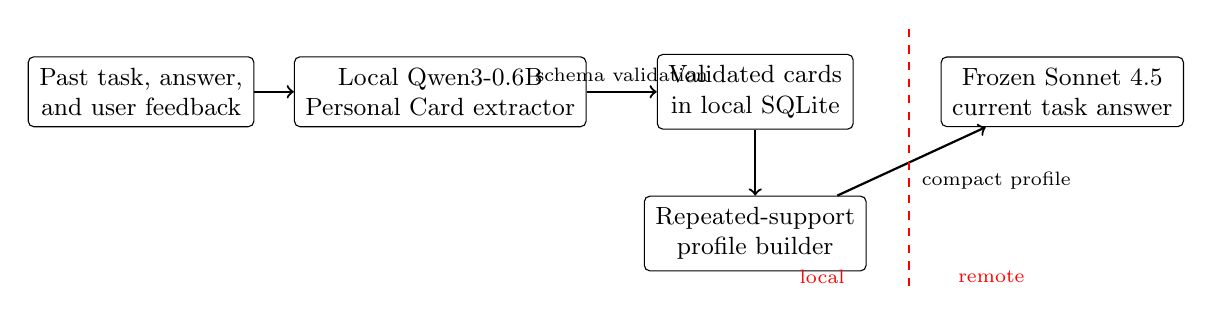
\begin{tikzpicture}[
  box/.style={draw, rounded corners=2pt, align=center, font=\small,
              minimum height=2.5em, inner sep=4pt},
  arr/.style={->, thick}
]
  \node[box] (history) at (0,0) {Past task, answer,\\and user feedback};
  \node[box] (extractor) at (3.8,0) {Local Qwen3-0.6B\\Personal Card extractor};
  \node[box] (store) at (7.8,0) {Validated cards\\in local SQLite};
  \node[box] (profile) at (7.8,-1.8) {Repeated-support\\profile builder};
  \node[box] (remote) at (11.7,0) {Frozen Sonnet 4.5\\current task answer};
  \draw[arr] (history) -- (extractor);
  \draw[arr] (extractor) -- node[above,font=\scriptsize] {schema validation} (store);
  \draw[arr] (store) -- (profile);
  \draw[arr] (profile) -- node[below right,font=\scriptsize] {compact profile} (remote);
  \draw[red,dashed,thick] (9.75,0.8) -- (9.75,-2.5);
  \node[red,font=\scriptsize] at (8.65,-2.35) {local};
  \node[red,font=\scriptsize] at (10.8,-2.35) {remote};
\end{tikzpicture}
}
\caption{The old conversation and card evidence stay local. The remote model
receives the current task and a compact profile derived from eligible cards.}
\label{fig:pipeline}
\end{figure}

\subsection{Personal Card Schema}

Each card is a JSON object with ten required fields:
\begin{itemize}
    \item \texttt{task\_type}: one of eight archive task classes;
    \item \texttt{feedback\_types}: a nonempty subset of fifteen facets;
    \item \texttt{direction}: \texttt{like}, \texttt{dislike}, or
    \texttt{uncertain};
    \item \texttt{likert}: an integer from 1 to 5;
    \item \texttt{confidence}: a value in $[0,1]$;
    \item \texttt{scope}: \texttt{global}, \texttt{task\_type}, or
    \texttt{task\_instance};
    \item \texttt{instruction}: a reusable instruction of at most 240
    characters;
    \item \texttt{evidence}: a short local explanation of at most 160
    characters;
    \item \texttt{evidence\_type}: the source class described below; and
    \item \texttt{privacy}: the constant \texttt{local\_only}.
\end{itemize}
The extractor emits the card only. It does not answer the task.

The evidence contract has three classes. An
\texttt{explicit\_correction} is a real corrective user message. A
\texttt{verified\_revision} is an assistant revision that passes a
deterministic check for the requested change; it is weaker than user approval.
A \texttt{category\_label} has no explicit preference evidence. Because every
schema field is required, an abstention card uses
\texttt{no\_explicit\_feedback}, direction \texttt{uncertain}, Likert 3,
confidence 0.4, scope \texttt{task\_instance}, and an instruction that says
not to infer a lasting preference. Such cards train abstention and are never
eligible for transfer.

\subsection{Offline Training}

The archive builder creates targets with deterministic local rules. Explicit
corrections produce negative examples. A revision is added as a weak positive
only when it passes the requested-change check. Category-only examples teach
task classification without a preference claim. Conversation IDs, rather
than rows, are assigned to train, validation, and test.

We freeze the Qwen3-0.6B backbone \citep{yang2025qwen3tr} and train LoRA
modules \citep{hu2022lora} on \texttt{q\_proj}, \texttt{k\_proj},
\texttt{v\_proj}, and \texttt{o\_proj}. Only target JSON tokens contribute
to the loss:
\begin{equation}
\mathcal{L}(\theta)
=-\frac{1}{|T_c|}\sum_{t\in T_c}
\log p_\theta(y_t\mid y_{<t},o),
\label{eq:sft}
\end{equation}
where $T_c$ indexes the card completion. Prompt and observation tokens remain
visible through attention but receive label $-100$ and do not enter the loss.

\subsection{Repeated-Support Profile}

The profile store first rejects category-only cards, cards with direction
\texttt{uncertain}, confidence below 0.65, and cards with
\texttt{task\_instance} scope. Each retained row stores a hash of the
conversation ID and the full observation. The hash identifies a source
record; records from the same conversation can still have different hashes.

For an exact instruction string $u$, let $H(u)$ be its distinct evidence
hashes. The support is
\[
\operatorname{supp}(u)=|H(u)|.
\]
The instruction is transferable only when
\begin{equation}
\operatorname{supp}(u)\geq 2.
\label{eq:support}
\end{equation}
The store ranks candidates by
\begin{equation}
s(u)=\sum_{i:u_i=u} \gamma_i w(e_i), \qquad
w(e_i)=
\begin{cases}
1,&e_i=\texttt{explicit\_correction},\\
0.5,&e_i=\texttt{verified\_revision},
\end{cases}
\label{eq:rank}
\end{equation}
where duplicate hashes contribute once. It then keeps at most three rules,
skipping a lower-ranked rule when it adds no feedback facet.

The rendered profile is a small JSON block. It contains the task type; each
selected instruction; its feedback facets, support count, mean confidence,
mean Likert value, and scope; and a policy stating that the current request
overrides the profile. It contains no raw conversation, card evidence
sentence, source hash, or conversation identifier. Thus the method minimizes
what is sent, but the derived profile is still personal information.

\section{Experimental Design}
\label{sec:design}

\subsection{Offline Data}

The dataset contains 914 examples from one user's archive. Table
\ref{tab:data} shows both evidence types and conversation-disjoint splits.

\begin{table}[t]
\centering
\caption{Offline dataset. Evidence counts and split counts describe different
partitions of the same 914 examples.}
\label{tab:data}
\begin{tabular}{lr}
\toprule
Item & Count \\
\midrule
Explicit corrections & 260 \\
Verified revisions & 39 \\
Category-only abstentions & 615 \\
\midrule
Train & 582 \\
Validation & 149 \\
Test & 183 \\
\bottomrule
\end{tabular}
\end{table}

\subsection{Card Extraction}

The LoRA adapter and untouched base model receive the same extraction prompt,
test examples, greedy decoding settings, and validator. We report valid-card
rate, task-type accuracy, direction accuracy, exact Likert accuracy, scope
accuracy, exact feedback-facet set accuracy, and pooled feedback micro F1.
An invalid output scores zero on all field metrics. The untouched model is a
format-and-task control, not a competitive instruction-tuned baseline.

\subsection{Cross-Session Transfer}

The first diagnostic applies one eligible card to one new task of the same
type. Its eight task IDs are then excluded from the main run.

For the main run, the local store is populated from the adapter predictions.
It holds 74 candidate rows after the per-card source, direction, confidence,
and scope filters. The case selector chooses eight new tasks from the separate
holdout file before the first executor call. It rejects tasks that depend on
missing attachments or surrounding context and alternates across task types
with available profiles.

For each task, Sonnet 4.5 answers once with the base system prompt and once with
the rendered profile appended to that prompt. The same model family judges
the pair twice with answer order reversed. The judge sees the current task,
the compact profile, and both candidate answers. It returns a winner and 1--5
scores for task quality and preference fit. A pair is position-consistent only
when both orderings select the same underlying answer.

We average the two judge orderings for each condition and compute paired
deltas. To show uncertainty, we resample the eight paired tasks 20,000 times
with seed 20260905 and report percentile 95\% intervals.

\section{Results}
\label{sec:results}

\subsection{H100 Training and Card Extraction}

Training uses four epochs, micro-batches of 2, gradient accumulation of 8,
rank 16, alpha 32, dropout 0, and learning rate $2\times10^{-4}$. The frozen
backbone has 4,587,520 trainable LoRA parameters. The raw training split has
582 examples. Repeating the 20 verified revisions in that split five times
produces 662 loader examples per epoch.

The run uses one NVIDIA H100 80GB HBM3. Training inside the process takes
260.76 seconds and reaches validation loss 0.0667. Peak allocated GPU memory
is 25.53 GiB. No training or validation example is truncated at the
4,096-token limit.

Table \ref{tab:extractor} gives held-out results. The adapter produces a valid
card for all 183 examples. Direction and evidence type are exact on every
example, while task-type and feedback-facet prediction remain the main error
sources. The untouched base model produces no valid card under this protocol.

\begin{table}[t]
\centering
\caption{Held-out Personal Card extraction on 183 examples.}
\label{tab:extractor}
\begin{tabular}{lrr}
\toprule
Metric & Base & LoRA \\
\midrule
Valid card JSON & 0.000 & 1.000 \\
Task-type accuracy & 0.000 & 0.705 \\
Direction accuracy & 0.000 & 1.000 \\
Likert exact accuracy & 0.000 & 0.831 \\
Scope accuracy & 0.000 & 0.995 \\
Feedback exact set & 0.000 & 0.639 \\
Feedback micro F1 & 0.000 & 0.732 \\
\bottomrule
\end{tabular}
\end{table}

\subsection{Single Cards Do Not Transfer Reliably}

The single-card diagnostic produces three guided wins, three baseline wins,
one tie, and one position-inconsistent pair. This gives no net advantage.
Manual inspection shows why: one correction can encode a file name, number, or
other detail that should not move to another task. This result motivated the
support threshold in Eq.\ \eqref{eq:support}.

\subsection{Repeated Support}

Table \ref{tab:online} reports the main run. The profile wins five of seven
position-consistent comparisons. Mean task quality is identical in the two
conditions. Mean preference fit is 0.625 points higher with the profile.

\begin{table}[t]
\centering
\caption{Repeated-support evaluation on eight new tasks. Deltas are profile
minus baseline.}
\label{tab:online}
\begin{tabular}{lr}
\toprule
Measure & Result \\
\midrule
Profile / baseline / inconsistent & 5 / 2 / 1 \\
Profile win rate among consistent pairs & 0.714 \\
Mean task quality, baseline / profile & 4.250 / 4.250 \\
Mean preference fit, baseline / profile & 3.375 / 4.000 \\
Paired task-quality delta & 0.000 \\
Paired preference-fit delta & $+0.625$ \\
95\% interval, task-quality delta & $[-0.6875,\ 0.5625]$ \\
95\% interval, preference-fit delta & $[-0.25,\ 1.5]$ \\
Mean latency, baseline / profile & 21.32 s / 26.24 s \\
Total executor and judge cost & \$1.923 \\
\bottomrule
\end{tabular}
\end{table}

\begin{figure}[t]
\centering
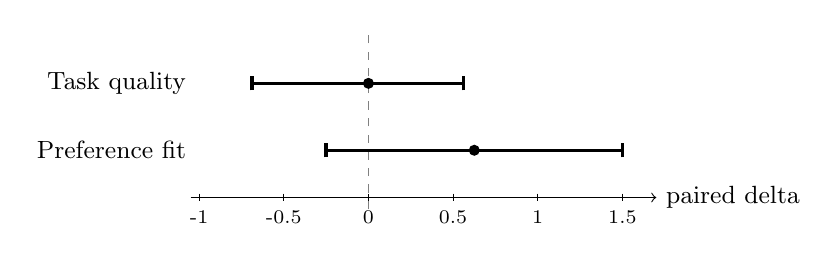
\begin{tikzpicture}[x=2.15cm,y=1.0cm]
  \draw[->] (-1.05,0) -- (1.7,0) node[right,font=\small] {paired delta};
  \foreach \x/\lab in {-1/-1,-0.5/-0.5,0/0,0.5/0.5,1/1,1.5/1.5}{
    \draw (\x,0.05)--(\x,-0.05) node[below,font=\scriptsize] {\lab};
  }
  \draw[dashed,gray] (0,-0.15)--(0,2.15);
  \draw[very thick] (-0.6875,1.45)--(0.5625,1.45);
  \draw[very thick] (-0.6875,1.36)--(-0.6875,1.54);
  \draw[very thick] (0.5625,1.36)--(0.5625,1.54);
  \fill (0,1.45) circle (2pt);
  \node[left,font=\small] at (-1.02,1.45) {Task quality};
  \draw[very thick] (-0.25,0.6)--(1.5,0.6);
  \draw[very thick] (-0.25,0.51)--(-0.25,0.69);
  \draw[very thick] (1.5,0.51)--(1.5,0.69);
  \fill (0.625,0.6) circle (2pt);
  \node[left,font=\small] at (-1.02,0.6) {Preference fit};
\end{tikzpicture}
\caption{Paired point estimates and 20,000-resample percentile intervals.
Both intervals include zero.}
\label{fig:intervals}
\end{figure}

The intervals in Figure \ref{fig:intervals} are wide and include zero. The
point estimates are consistent with improved preference fit without lower mean
task quality, but they do not establish a reliable effect. We report this as
feasibility evidence.

The profile adds 4.93 seconds of mean executor latency in this run. The complete
main evaluation uses 16 executor calls and 16 judge calls and costs
\$1.923. These measurements describe this task set and profile length; they do
not identify the cause of the latency difference.

\subsection{Failure Analysis}

The manual audit identifies clear profile wins on repository upload
instructions, a short translation, campaign questions, and a Newton
convergence explanation. It also finds three different failure modes.

First, the guided least-squares answer states that its displayed data sum to
54, although they sum to 53. More detailed structure did not protect against
arithmetic error. Second, both answers to the degrees-of-freedom question are
too broad and can leave a false impression about known variance. The profile
cannot repair an error shared by the executor. Third, the foreign-key pair
changes winner when answer order is reversed. That pair is reported as
position-inconsistent rather than forced into a win or loss.

We also tried a Qwen2.5-7B-Instruct teacher that rewrote individual corrections
as broader rules. We cancelled the branch after 216 labels: 201 had
\texttt{task\_instance} scope, and 9 were deterministic fallbacks after invalid
model output. No student model was trained from these labels. This is a failed
engineering branch, not an ablation result.

\section{Discussion and Limitations}
\label{sec:discussion}

The offline result is the strongest part of the study. A 0.6B local model can
learn the card schema and abstention behavior in a few GPU minutes. Its task
classification accuracy, however, is only 0.705. Since task type routes a card
to a profile bucket, these errors can split support across the wrong buckets.
The 0.639 exact feedback-set accuracy can also change which rules survive facet
deduplication.

Repeated support is useful because it provides a clear transfer gate. It does
not solve semantic equivalence: two paraphrases count as different
instructions. The failed 7B branch shows that learned rewriting can
over-generalize or copy one-off details, but our current exact-string rule can
under-generalize. A future method should cluster paraphrases while preserving
source-level auditability.

The online stage changes local memory, not model weights. It therefore supports
fast profile updates but does not test online fine-tuning. The benchmark also
has one user and eight tasks. Sonnet 4.5 acts as executor and judge, and the
judge sees the same profile used to guide one answer. Preference fit therefore
measures compliance with the displayed profile, not independent user
satisfaction. Human judgments and a cross-family judge are needed before
making a stronger claim.

Finally, ``local'' does not mean private in a formal sense. Raw history and
evidence text stay on the user's machine, but support counts, confidence,
Likert summaries, facets, and derived instructions are sent to the remote
model. We provide no differential-privacy or cryptographic guarantee
\citep{dwork2006calibratingnt}. The source archive is also private and cannot
be released without review and consent, which limits exact external
reproduction. Persistent profiles require clear user controls for inspection
and deletion before deployment.

\section{Conclusion}

We built and tested a complete path from one user's historical corrections to
a local Personal Card store and then to a frozen remote model. The local
extractor is cheap and reliably emits valid structured cards. Single-card
transfer fails, while repeated support gives a positive but uncertain signal
on eight new tasks. The result is a working, auditable feasibility prototype.
The next evidence should come from more users and tasks, stronger extractor
baselines, and independent judges rather than from stronger wording around the
current numbers.

\appendix

\section{Exact Data and Schema Details}
\label{app:data}

\subsection{Task and Feedback Vocabularies}

The eight task values in the implementation are
\texttt{knowledge explanation}, \texttt{proof/problem solving},
\texttt{code development}, \texttt{operations/troubleshooting},
\texttt{format processing}, \texttt{writing/editing},
\texttt{research analysis}, and \texttt{planning}. The stored enum values are
the corresponding Chinese labels used by the source archive.

The fifteen feedback facets are:
\texttt{verbosity}, \texttt{detail\_depth}, \texttt{format\_structure},
\texttt{tone\_style}, \texttt{language}, \texttt{correctness},
\texttt{constraint\_adherence}, \texttt{context\_memory},
\texttt{clarification}, \texttt{tool\_use},
\texttt{workflow\_compliance}, \texttt{code\_runnability},
\texttt{source\_verification}, \texttt{task\_success}, and
\texttt{no\_explicit\_feedback}.

\subsection{Evidence Counts by Split}

\begin{table}[h]
\centering
\caption{Evidence type within each conversation-disjoint split.}
\label{tab:evidence-split}
\begin{tabular}{lrrrr}
\toprule
Evidence & Train & Validation & Test & Total \\
\midrule
Explicit correction & 146 & 51 & 63 & 260 \\
Verified revision & 20 & 7 & 12 & 39 \\
Category label & 416 & 91 & 108 & 615 \\
\midrule
Total & 582 & 149 & 183 & 914 \\
\bottomrule
\end{tabular}
\end{table}

\subsection{Validation}

The Python validator checks the task and feedback enums, direction, Likert
range, confidence range, scope, nonempty instruction and evidence strings,
their length limits, evidence type, and the \texttt{local\_only} privacy
constant. The prediction parser accepts a JSON object found in the completion
and then applies this validator. Invalid cards are recorded as failed
predictions and never enter the profile store.

\section{Training Configuration}
\label{app:training}

\begin{table}[h]
\centering
\caption{Offline SFT configuration.}
\label{tab:training}
\begin{tabular}{ll}
\toprule
Setting & Value \\
\midrule
Backbone & Qwen3-0.6B, frozen \\
LoRA targets & \texttt{q\_proj}, \texttt{k\_proj}, \texttt{v\_proj}, \texttt{o\_proj} \\
Rank / alpha / dropout & 16 / 32 / 0 \\
Trainable parameters & 4,587,520 \\
Epochs & 4 \\
Learning rate & $2\times10^{-4}$ \\
Micro-batch / accumulation & 2 / 8 \\
Optimizer & AdamW, weight decay 0.01 \\
Schedule & cosine, 6\% warmup \\
Precision & bfloat16 \\
Maximum sequence length & 4,096 \\
Verified-revision repetition & 5 \\
Random seed & 17 \\
\bottomrule
\end{tabular}
\end{table}

\section{Per-Task Online Results}
\label{app:tasks}

\begin{table}[h]
\centering
\small
\caption{Main online run. Score deltas are profile minus baseline after
averaging the two judge orderings.}
\label{tab:tasks}
\begin{tabular}{lcrr}
\toprule
Task & Verdict & $\Delta$ quality & $\Delta$ preference \\
\midrule
Booth naming & baseline & $-0.5$ & $-0.5$ \\
Repository upload & profile & $+1.0$ & $+0.5$ \\
Degrees of freedom & profile (weak) & $+1.0$ & $0.0$ \\
Short translation & profile & $+0.5$ & $+2.0$ \\
Least squares & baseline & $-2.0$ & $-1.5$ \\
Campaign questions & profile & $-0.5$ & $+2.5$ \\
Newton convergence & profile & $+0.5$ & $+1.5$ \\
Foreign-key guidance & inconsistent & $0.0$ & $+0.5$ \\
\bottomrule
\end{tabular}
\end{table}

The manual audit does not replace a blind human study. It labels the
repository, translation, campaign, and Newton cases as clear profile wins. The
degrees-of-freedom win is weak because both answers are potentially
misleading. Booth naming and least squares are clear baseline wins. The
foreign-key pair remains unresolved.

\section{Artifact Map and Next Experiments}
\label{app:artifacts}

\begin{table}[h]
\centering
\small
\caption{Authoritative local artifacts.}
\label{tab:artifacts}
\begin{tabular}{p{4.2cm}p{7.4cm}}
\toprule
Artifact & Content \\
\midrule
\path{data_balanced_v2/dataset_manifest.json} &
dataset size, source counts, split counts, and disjointness flag \\
\path{outputs/qwen3_0p6b_personal_card_balanced_v2/} &
adapter, training summary, base and adapter predictions, extraction metrics \\
\path{outputs/online_sonnet45_balanced_v2/} &
single-card diagnostic protocol, answer pairs, and summary \\
\path{outputs/online_sonnet45_repeated_profile_v2/} &
main protocol, SQLite profile, answer pairs, paired metrics, and manual audit \\
\path{outputs/archive_local_teacher_failed_scope_20260905/} &
cancelled 7B teacher branch and failure record \\
\bottomrule
\end{tabular}
\end{table}

The next experiments are intentionally left open rather than reported as
results:
\begin{enumerate}
    \item repeat both tracks on another consenting user's archive;
    \item judge the stored answer pairs with blinded humans and another model
    family;
    \item compare the LoRA extractor with an instruction-tuned zero-shot
    extractor under the same schema and metrics;
    \item freeze a larger set of new tasks before generation and rerun the
    paired protocol;
    \item test semantic grouping of paraphrased rules while retaining distinct
    source support and an auditable transfer log.
\end{enumerate}

\bibliography{iclr2026_conference}
\bibliographystyle{iclr2026_conference}

\end{document}
